%\documentclass[PhD]{iitmdiss}
%\documentclass[MS]{iitmdiss}
%\documentclass[MTech]{iitmdiss}
%\documentclass[BTech]{iitmdiss}
\documentclass[DD]{iitmdiss}
\usepackage{times}
 \usepackage{t1enc}

\usepackage{graphicx}
%\usepackage{epstopdf}
\usepackage[driverfallback=dvipdfm]{hyperref} % hyperlinks for references.
\usepackage{amsmath} % easier math formulae, align, subequations \ldots

\begin{document}

%%%%%%%%%%%%%%%%%%%%%%%%%%%%%%%%%%%%%%%%%%%%%%%%%%%%%%%%%%%%%%%%%%%%%%
% Title page

\title{Infrastructure Agnostic\\
	 Cloud Computing Platform for Programming Education}

\author{Muhammed Shahidh K, ED12B031}

\date{MAY 2017}
\department{ENGINEERING DESIGN}

%\nocite{*}
\maketitle

%%%%%%%%%%%%%%%%%%%%%%%%%%%%%%%%%%%%%%%%%%%%%%%%%%%%%%%%%%%%%%%%%%%%%%
% Certificate
\certificate

\vspace*{0.5in}

\noindent This is to certify that the thesis titled {\bf Infrastructure Agnostic Cloud Computing Platform for Programming Education}, submitted by {\bf Muhammed Shahidh K, ED12B031}, 
  to the Indian Institute of Technology, Madras, for
the award of the dual degree of {\bf Bachelor of Technology and Master of Technology}, is a bona fide
record of the research work done by him under our supervision.  The
contents of this thesis, in full or in parts, have not been submitted
to any other Institute or University for the award of any degree or
diploma.

\vspace*{1.5in}

\begin{singlespacing}
\hspace*{-0.25in}
\parbox{2.5in}{
\noindent {\bf Dr.~Gaurav~Raina} \\
\noindent Research Guide \\ 
\noindent Assistant Professor \\
\noindent Dept. of Electrical Engineering\\
\noindent IIT Madras, 600036 \\
} 
\hspace*{1.0in} 
\parbox{2.5in}{
\noindent {\bf Dr.~Asokan~Thondiyath} \\
\noindent Research Guide \\ 
\noindent Professor \\
\noindent Dept. of Engineering Design\\
\noindent IIT Madras, 600036 \\
}  
\end{singlespacing}
\vspace*{0.25in}
\noindent Place: Chennai\\
Date: 21st May 2017 


%%%%%%%%%%%%%%%%%%%%%%%%%%%%%%%%%%%%%%%%%%%%%%%%%%%%%%%%%%%%%%%%%%%%%%
% Acknowledgements
\acknowledgements

<will update>

%%%%%%%%%%%%%%%%%%%%%%%%%%%%%%%%%%%%%%%%%%%%%%%%%%%%%%%%%%%%%%%%%%%%%%
% Abstract

\abstract

\noindent KEYWORDS: \hspace*{0.5em} \parbox[t]{4.4in}{Cloud Computing, Virtualisation, Docker, Kubernetes, Education, Programming}

\vspace*{24pt}

\noindent The project showcases a scalable online programming platform which can be used to teach computer programming languages to students, by just using a web browser. The underlying architecture and use of virtualisation technology makes the platform infrastructure agnostic and hence can be deployed on to any cloud provider as well as bare metal. Using container runtime environments such as Docker, the platform can be configured to run any programming language and library. Further a PoC was developed and deployed for nearly 1,00,000 users for India's biggest MOOC (Massive Online Open Course) - IMAD (Introduction to Modern Application Development).

\pagebreak

%%%%%%%%%%%%%%%%%%%%%%%%%%%%%%%%%%%%%%%%%%%%%%%%%%%%%%%%%%%%%%%%%
% Table of contents etc.

\begin{singlespace}
\tableofcontents
\thispagestyle{empty}

\listoftables
\addcontentsline{toc}{chapter}{LIST OF TABLES}
\listoffigures
\addcontentsline{toc}{chapter}{LIST OF FIGURES}
\end{singlespace}


%%%%%%%%%%%%%%%%%%%%%%%%%%%%%%%%%%%%%%%%%%%%%%%%%%%%%%%%%%%%%%%%%%%%%%
% Abbreviations
\abbreviations

\noindent 
\begin{tabbing}
xxxxxxxxxxx \= xxxxxxxxxxxxxxxxxxxxxxxxxxxxxxxxxxxxxxxxxxxxxxxx \kill
\textbf{IITM}   \> Indian Institute of Technology, Madras \\
\textbf{MOOC} \> Massive Online Open Course \\
\end{tabbing}

\pagebreak

%%%%%%%%%%%%%%%%%%%%%%%%%%%%%%%%%%%%%%%%%%%%%%%%%%%%%%%%%%%%%%%%%%%%%%
% Notation

\chapter*{\centerline{NOTATION}}
\addcontentsline{toc}{chapter}{NOTATION}

\begin{singlespace}
\begin{tabbing}
xxxxxxxxxxx \= xxxxxxxxxxxxxxxxxxxxxxxxxxxxxxxxxxxxxxxxxxxxxxxx \kill
\textbf{$r$}  \> Radius, $m$ \\
\textbf{$\alpha$}  \> Angle of thesis in degrees \\
\textbf{$\beta$}   \> Flight path in degrees \\
\end{tabbing}
\end{singlespace}

\pagebreak
\clearpage

% The main text will follow from this point so set the page numbering
% to arabic from here on.
\pagenumbering{arabic}


%%%%%%%%%%%%%%%%%%%%%%%%%%%%%%%%%%%%%%%%%%%%%%%%%%
% Introduction.

\chapter{INTRODUCTION}
\label{chap:intro}
The skill of programming is considered fundamental and very important, making it a core requirement for all kinds of 21st century jobs. It is considered as basic literacy in the digital age. Programming education has long been part of engineering curriculum at university level and in the last decade or so at school level too. Traditionally programming is taught as a theory and lab course, where instructor teaches fundamentals in class and students get to apply what they learned in form of exercises and programming assignments. Typically, computer labs are used for these requirements.  

But, when the strength of students increase, like in case of a MOOC, where the numbers typically goes into the scale of thousands and lakhs, the traditional way is not the best. Using internet technologies, we have reach to millions of prospective learners. Here, we explore the possibilities to use recent technological advancements and solve the problems of flexibility and scale by building a programming environment in the cloud.

Modern day education sector is using cloud technologies for various aspects like hosting video lectures in YouTube, sharing files using Dropbox and Google Drive, collaborative document editing using Google Docs etc. These cloud based technologies enable access to online services anywhere and promises scalability, enhanced availability and cost savings.

This project is aimed at creating an online interface where instructors can create environments for various programming languages and users can write code in that environment, execute and view the results. The emphasis is given on flexibility to support any programming language and scalability to handle any number of users, using cloud computing techniques.
\section{Literature Review}
A state-of-the-art survey paper by \cite{gonzalez-martinez_cloud_2015} on cloud computing and education reviewed 112 works relevant to the field discuss various innovations, opportunities, shortcomings and risks.

While there are services like \cite{codeanywhere} which offers an IDE on the browser, none of them are open source and are not available for free.

\section{Outline of the Problem}

While there are plenty of programming languages and environments available, setting them up can be bit of a hurdle, especially in an educational institution environment where the class strengths are very high. If we look at the scenario of a typical introductory programming course at an undergraduate university, most of the students attending will be programming for the first time. When class strength is huge, it is not easy to have the infrastructure or the man power to manage computer labs. 

Especially at times when many MOOCs are offered online, getting everybody to code in a computer lab is not possible. Most of the students have their own devices, which can access internet. If we go with traditional way of installing environment to write, compile or interpret and run programs, this will prove to be quite tedious. First of all, all users might not be aware or comfortable with the tools or background knowledge required to install these programs. On top of that, considering the wide variety of devices and their operating systems, like Windows, Linux (which in-turn has many distributions), MacOS, Android, iOS, ChromeOS etc., providing instructions for everyone is very difficult for the instructor. Also, if user is on a mobile OS, like a tablet, there is absolutely no way of them installing programs that let them code. Finally, everyone's device and the environment is different. If there are some dependency errors etc, fixing them would take precious time for learning.

A student/user should be spending their time on learning the language, its syntax and usages. They should not be wasting time on installing, fixing and configuring tools and environments to run their code. This can have a negative effect on beginners who are just getting into programming. Students could get frustrated and leave the course.

\subsection{Usability}
This is the primary problem that is being addressed here. There should be an easy to use programming interface that would work the same on every device. Only a web application can be made to work like this through a web browser. Being a web application, the program can be served through internet and be made available anytime anywhere. By leveraging cloud computing along with virtualisation and containerisation technologies, millions of users can write code and run their programs.

\subsection{Flexibility}
The second problem being tackled is compatibility with any programming language. Course instructors should be able to create any kind of environment for their students to code in, with minimal effort. The platform should not be restrictive in any manner to create preferred environment. Students should be able to code and run their programs against these pre-defined environments. At the same time, if required, students should be able to modify and create their own environments so that the explorer's curiosity is not hindered.

Flexibility also implies that the platform should be able to run on any infrastructure. Public and private clouds, bare metal servers, normal desktop/laptops etc. should be able to host the platform. The only disadvantage of running on a non-cloud infrastructure should be trade-offs with scalability.

\subsection{Scalability}
Third issue being considered is scalability of the platform. With minimal or preferably no effort, the platform should be scalable to support any number of users. We are targeting a hundred thousand users for the PoC. 

\subsection{Security}
Each user's code should be secure and isolated. Unauthorized access should be prevented and measures have to be taken to prevent attacks like DDoS or MitM.

\chapter{EVALUATION METHODOLOGY}
%Includes how the student intends to tackle the problem, avenues for investigation, possible milestones, options for different architectures, etc. [3-4 pages]

A web application is best served for the purpose, since the only requirement is a web browser and internet connection. This will very well serve the usability requirement since a common interface is exposed through a web browser and all modern consumer devices support web browsers. Flexibility to create any programming environment can be attained using containers. LXC, Docker and Rocket are some of the popular container runtime environments. Even though there are performance trade-off by using containers \citep{ruan_performance_2016}, the flexibility and easiness to create any environment will surpass it.

Choosing the correct container runtime is important to make the platform user friendly. Popular runtimes tend to have more documentation and support for all kinds of programs. In order to determine popularity, tech firms in the computer science industry were consulted and by word of mouth Docker emerged to be a clear winner. In order to further back this up, a Google Trends analysis carried out between Docker, LXC and Rocket \citep{google_trends_docker_lxc_rkt} is shown in Fig.~\ref{fig:google_trends_docker_rkt_lxc}. 

\begin{figure}
\centering
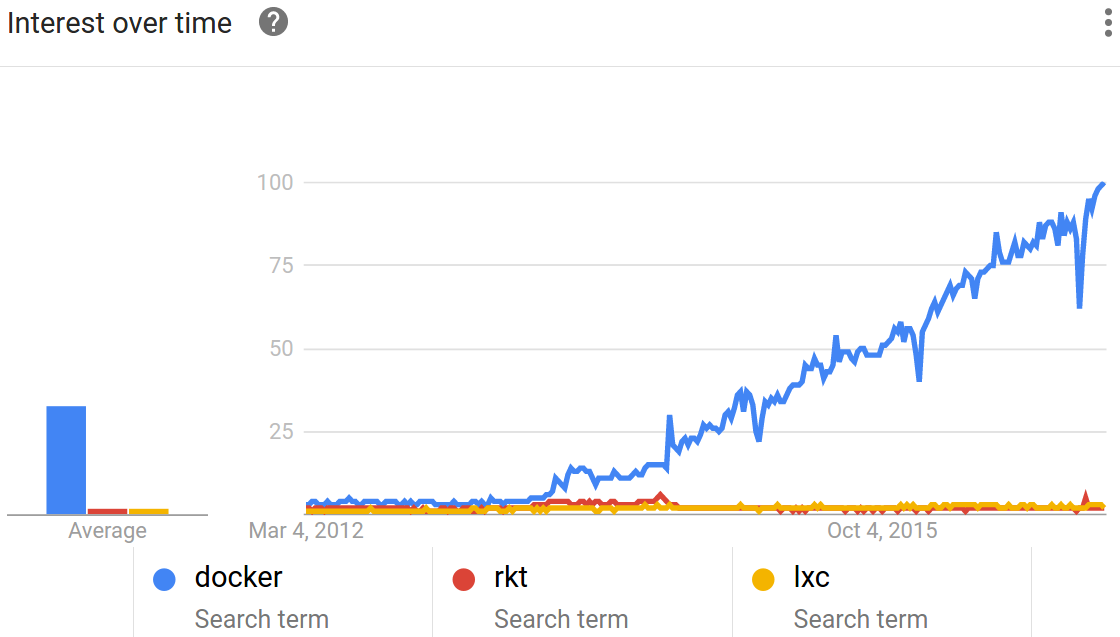
\includegraphics[width=0.7\linewidth]{img/google_trends_docker_rkt_lxc}
\caption[Google Trends for docker, rkt, lxc]{Google Trends for docker, rkt, lxc - wordwide, past 5 years, retrieved on 2017-02-27}
\label{fig:google_trends_docker_rkt_lxc}
\end{figure}


\chapter{RESULTS}
(i) progress made, (ii) results, (iii) sample code, (iv) refinement of the problem statement, and (v) potential work outline for the next 2-3 months. This will count for 25% of the final grade.                

Upgrade the report of Stage 1, and add another chapter say called Results, which includes progress made, and the potential work outline for the next 2-3 months
%%%%%%%%%%%%%%%%%%%%%%%%%%%%%%%%%%%%%%%%%%%%%%%%%%%%%%%%%%%%
% Appendices.

\appendix

\chapter{SOURCE CODE}

All source code is present in GitHub. Links are given here.

%%%%%%%%%%%%%%%%%%%%%%%%%%%%%%%%%%%%%%%%%%%%%%%%%%%%%%%%%%%%
% Bibliography.

\begin{singlespace}
	\bibliography{refs}
\end{singlespace}


%%%%%%%%%%%%%%%%%%%%%%%%%%%%%%%%%%%%%%%%%%%%%%%%%%%%%%%%%%%%
% List of papers

\listofpapers

\begin{enumerate}  
\item Authors....  \newblock
 Title...
  \newblock {\em Journal}, Volume,
  Page, (year).
\end{enumerate}  

\end{document}
